% Position Calculation


\chapter{Position Calculation} % Main chapter title

\label{PositionCalculation}

%----------------------------------------------------------------------------------------

\section{Overview}
%Talk about the goal of this section: to calculate positions of objects given the ranges between them. Talk about how Arduinos and Androids are connected by FTDI.

Our location tracking system consists of two different anchors, anchors and tags. The anchors which we can think of as static anchors doing the postion tracking, and the tags which are our dynamic anchors that we need to track. The overall goal of this subsystem is to calculate the position of each anchor given only the distances from one another.
The anchors use ultrawideband technolgy to communicate with each other and send the position data to our android application using FTDI.


\section{High-Level Example in 2D}
To start the position calculation we take three different anchors for example $a_{0}$, $ a_{1}$  and $a_{2}$. We set an arbitrary point as the origin $a_{0}$, then we proceed to make a horizontal line from $a_{0}$ to another anchor say $a_{1}$, since we have all the distances between the anchors we can now use basic trigonometry to calculate the position of our last anchor $a_{2}$.
An Example calculation is as follows:
\\\\
distance from anchor x to anchor y: $d_{xy}$, we use cosine law to determine the angle
\\
\[ \Theta = \cos ^{ - 1}\Big(\frac{d_{01}^2 + d_{02}^2 - d_{12}^2 }{2*d_{01}*d_{02}}\Big)\]
\\
when we have the angle we can now calculate the x and y coordinates:
\\
\[ x_2 = cos(\Theta) * d_{12} \]
\[ y_2 = sin(\Theta) *  d_{12} \]

\section{Extending This to 3D}
Extending the subsystem to three dimensions does not really change the calculation all that much except that we now need four anchors to get a reliable position in three dimensions. We have our four anchors: $a_{0}$, $a_{1}$ , $a_{2}$ and $a_{3}$, we arbitrarily set one as the origin $a_{0}$(0, 0, 0) and we now make a horizontal line to another anchor say $a_{1}$ and since we know the distance between these two anchors we can get the position to be $a_{1}$(0, $d_{01}$, 0), where $d_{01}$ is the distance between $a_{0}$ and $a_{1}$. We can now form a triangle with the third anchor and use cosine law to determine the position and we arbitrarily set the z value to 0.
\\
We now have the coordinates for the third anchor, but we do not know the correct orientation in the z axis, it could be either positive or negative. This is where the fourth anchor comes in, we use the anchor to create a temporary point using the same method we use above.
\\
\[ \Theta = \cos ^{ - 1}\Big(\frac{d_{01}^2 + d_{03}^2 - d_{13}^2 }{2*d_{01}*d_{03}}\Big)\]
\\
\[ x_{temp} = cos(\Theta) * d_{13} \]
\[ y_{temp} = sin(\Theta) *  d_{13} \]
\[ z_{temp} = 0 \]
\\
We will rotate around the x-axis by keeping the x value constant and taking the y distance and z distance to be a circle of radius of $y_{temp}$.We calculate the distance between the x value of the temporary point and the x value of anchor 2, we denote this value $\Delta x$.
\\
\[ \Delta x = x_{temp} - x_{2} \]
\\
Now that we have $\Delta x$ we can now calculate the position of our fourth anchor using cosine law.
\\
\[\Theta = \cos ^{ - 1}\Big(\frac {\Delta x^2 - d_{23}^2 + y_{2}^2 + y_{temp}^2}{2*y_{2}*y_{temp}}\Big)\]
\\
\[ x_{3} = x_{temp} \]
\[ y_{3} = cos(\Theta) * y_{temp} \]
\[ z_{3} = sin(\Theta) * y_{temp} \]


\section{Arbitrariness (pick a better title later)}
The positions calculated from ranges do not correspond to the real world! We must use the cellphones' accelerometer (for gravity) and magnetic sensor (for compass direction/inclination) to map these positions to reality.

Go over how this is done.

\section{Getting the Ranges}
Talk about FTDI and our protocol to communicate from Arduino to Android. Go over how they are parsed (put in appendix of parsing code)

\section{Conclusion}
This subsystem calculates positions; we figured out how ranges are obtained, how they are calculated. Go over this in more detail.

\begin{figure}
\section{Proof}
	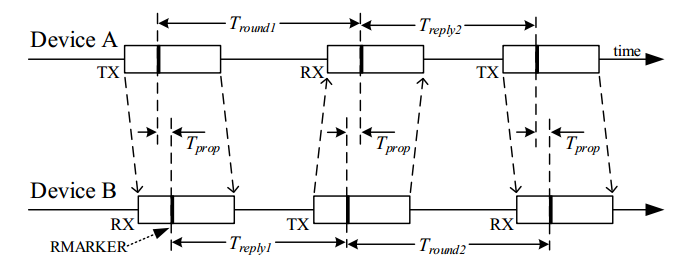
\includegraphics[width=\linewidth]{tprop.png}
	\caption{Double-sided Two-way ranging with three messages}

We begin by assuming that the clock of one node is off by alpha ($\alpha$) and the other by beta ($\beta$), the key here was to find the time of flight in a virtual clock that would be the mean value of alpha and beta.
\\
\[ \alpha a = 2t + \beta c  \tag{1} \label{eq:1} \]
\[ \beta d = 2t + \alpha b  \tag{2} \label{eq:2} \]
\[ 1 = \frac{\alpha + \beta}{2} \]
\\
We simplify and solve for $\beta$:
\\
\[ \beta = 2 - \alpha  \tag{3} \label{eq:3} \]
\\
We then subsititute equation \eqref{eq:3} into equation \eqref{eq:1} and equation \eqref{eq:2}.
\\
\[ \alpha a = 2t + 2c - \alpha c  \tag{4} \label{eq:4} \]
\[ 2d - \alpha d = 2t + \alpha b  \tag{5} \label{eq:5} \]
\\
Isolate $\alpha$ for both equations \eqref{eq:4} and \eqref{eq:5} we get the following:
\\
\[ \alpha = \frac{2(t + c)}{a + c}  \tag{4.1} \label{eq:4.1} \]
\[ \alpha = \frac{2(d - t)}{b + d}  \tag{5.1} \label{eq:5.1} \]
\\
Setting \eqref{eq:4.1} and \eqref{eq:5.1} equal to each other we can solve for propagation time, t.
\\
\[ 2(t + c)(b +d) = 2(d - t)(a + c)\]
\[ tb + td +bc + dc = da + dc - ta - tc \]
\[ t(b + d + a + c) = da - bc\]
\[ t = \frac{da-bc}{a + b + c + d}  \tag{6} \label{eq:6} \]
\\
\end{figure}
